%%%%%%%%%%%%%%%%%%%%%%%%%%%%%%%%%%%%%%%%%%%%%%%%%
%%%%%  make FCCeeParis14.pdf
%%%%%%%%%%%%%%%%%%%%%%%%%%%%%%%%%%%%%%%%%%%%%%%%%
\documentclass{beamer}
%\documentclass[handout]{beamer}


\mode<presentation>
{
  \usetheme{Warsaw}
 %\usetheme{Hannover}
  \setbeamercovered{transparent}
}

\usepackage[english]{babel}
\usepackage{xcolor}
\usepackage[latin1]{inputenc}

\usepackage{times}
\usepackage[T1]{fontenc}
\usepackage{listings}
%------------------------------------------------------
\usepackage{amsbsy}
\usepackage{amsmath,amssymb,bbm}
\usepackage{euscript}
\usepackage{fancybox}


%%%%%%%%%%%%%%%%%%%%%%%%%%%%%%%%%%%%%%%%%%%%%%%%%%%%%%%%%%%%%%%
%%% Macros 
\newcommand{\Pcal}{{\cal P}}
\newcommand{\Kcal}{{\cal K}}
\newcommand{\Dcal}{{\cal D}}
%
\newcommand{\Peu}{\EuScript{P}}
\newcommand{\Keu}{\EuScript{K}}
\newcommand{\Deu}{\EuScript{D}}
\newcommand{\Reu}{\EuScript{R}}
\newcommand{\Feu}{\EuScript{F}}
%
\newcommand{\Pmf}{\mathfrak{P}}
\newcommand{\Dmf}{\mathfrak{D}}
%
\newcommand{\Pbbm}{\mathbbm{P}}
\newcommand{\Rbbm}{\mathbbm{R}}
\newcommand{\Zbbm}{\mathbbm{Z}}
\newcommand{\Bbbm}{\mathbbm{B}}
\newcommand{\Pop}{\overleftarrow{\Pbbm}}
\newcommand{\Zop}{\overleftarrow{\Zbbm}}
\newcommand{\Bop}{\overleftarrow{\Bbbm}}
\newcommand{\Rop}{\overleftarrow{\Rbbm}}
%
\newcommand{\Tbf}{\mathbf{T}}
\newcommand{\Pbf}{\mathbf{P}}
\newcommand{\Dbf}{\mathbf{D}}
\newcommand{\Phibf}{\mathbf{\Phi}}
%
\newcommand{\udl}{\underline}
\newcommand{\from}{\leftarrow}
\newcommand{\bu}{\bullet}
\newcommand{\veps}{\varepsilon}
\newcommand{\Dyfs}{D_{_{\rm YFS}}}
\newcommand{\tH}{{\hat{t}}}
\newcommand{\tB}{{\bar{t}}}
\newcommand{\tBl}{{\bar{t}_\lambda}}
% boldfaces and vectors
\newcommand{\ba}{{\bf{a}}}
\newcommand{\bk}{{\bf{k}}}
\newcommand{\vkap}{{\vec{\kappa}}}
\newcommand{\vrk}{{\varkappa}}
\newcommand{\alfb}{{\bar{\alpha}}}
\newcommand{\betb}{{\bar{\beta}}}


\newcommand{\cbl}{\color{blue}}
\newcommand{\crd}{\color{red}}
\newcommand{\cmg}{\color{magenta}}
\newcommand{\cgr}{\color{green}}
\newcommand{\cwh}{\color{white}}
\newcommand{\yel}{\color{yellow}}
\newcommand{\blk}{\color{black}}
\newcommand{\cya}{\color{cyan}}

\newcommand{\ns}{\normalsize}

%%%%%%%%%%%%%%%%%%%%%%%%%%%%%%%%%%%%%%%%%%%%%%%%%%%%%%%%%%%%%%%%%%
%%%%%%%%%%%%%%%%%%%%%%%%%%%%%%%%%%%%%%%%%%%%%%%%%%%%%%%%%%%%%%%%%%
%%%%%%%%%%%%%%%%%%%%%%%%%%%%%%%%%%%%%%%%%%%%%%%%%%%%%%%%%%%%%%%%%%
%%%%%%%%%%%%%%%%%%%%%%%%%%%%%%%%%%%%%%%%%%%%%%%%%%%%%%%%%%%%%%%%%%
\title[Precision Monte Carlo generators] % (optional)
{ {\bf Precision event generators for EW physics}
} % (optional)


\author[S.~Jadach] % (optional, use only with lots of authors)
{\Large\bf S.~JADACH }


\institute[Universities of Somewhere and Elsewhere] % (optional)
{ {\large\crd IFJ-PAN, Krak\'ow, Poland}\\
  {~~~}\\
  {\footnotesize
  Partly supported by Polish Government grant\\
  {\em Narodowe Centrum Nauki} DEC-2011/03/B/ST2/02632
}}

\date[Short Occasion] % (optional)
{\small FCCee physics workshop\\
   Paris, October 27-29th, 2014
\vskip 4mm
 \footnotesize
  More material on http://192.245.169.66:8000/FCCeeMC/wiki
}

\subject{Talks}
% only for the PDF information catalog.

\pgfdeclareimage[height=0.5cm]{university-logo}{ifj}
\logo{\pgfuseimage{university-logo}}


\begin{document}

\begin{frame}
  \titlepage
\end{frame}


%----------------------------------------------------------------
%----------------------------------------------------------------
\begin{frame}[fragile]
\frametitle{\bf Outline}

\vspace{2mm}
\large\cbl
Three subjects/parts:
\begin{itemize}
\item\cbl
 Main points (updates) of previous talk on prec. MCs
\item
 New wiki page of MC generators for FCCee\\
 (mostly undusted LEP codes)
\item
 Update on invisible Z width from radiative return
\end{itemize}
\end{frame}

%----------------------------------------------------------------
%----------------------------------------------------------------
\begin{frame}[fragile]
\frametitle{\bf Precision Monte Carlo event generators}

\vspace{-3mm}
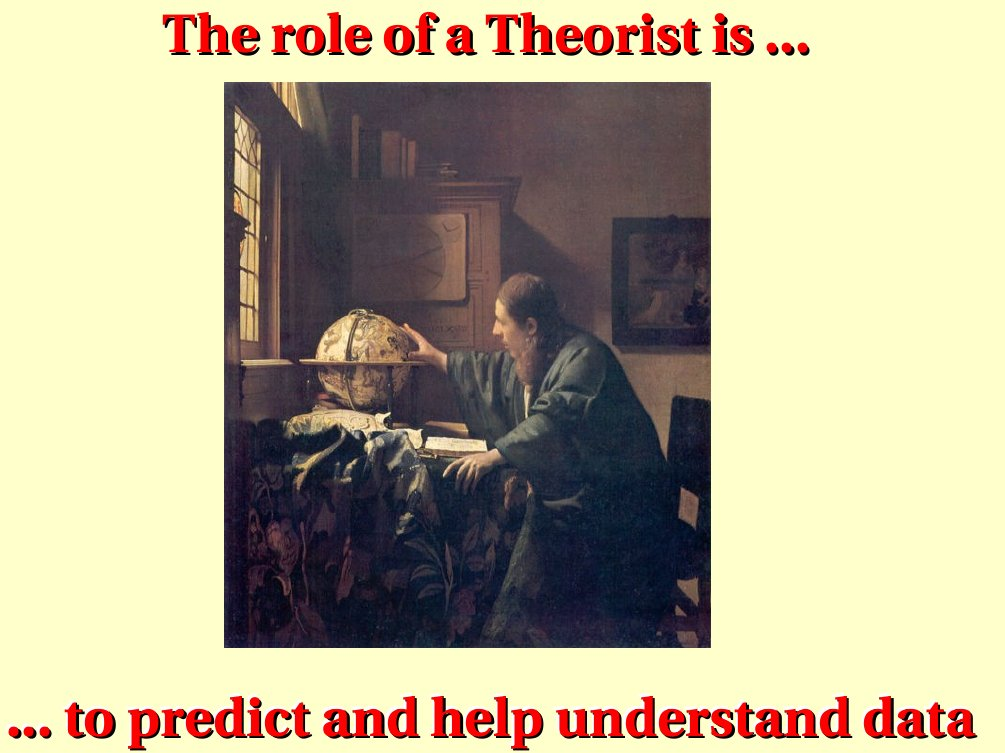
\includegraphics[width=60mm]{./sli0.jpg}

\begin{itemize}
\item\cbl
 Theoretical predictions with precision $\leq 1\%$.
\item
 Real and virtual diagram contributions
\item
 All kind of non-factorisable contribution not the problem
\item
 Can handle arbitrary experimental cuts/selection
\item
 Soft-collinenar photon resummations in exclusive form
\item
 But very costly in the developement, precision validation!\\
 hence mostly for known physics, like SM
\item
 Most of LEP-era precision MC appeared after LEP start!!!
\end{itemize}
\
\end{frame}

%
%----------------------------------------------------------------
%----------------------------------------------------------------
\begin{frame}[fragile]
\frametitle{\bf\ns 
 Main points from CERN June 2014 talk on precision MCs for FCCee}

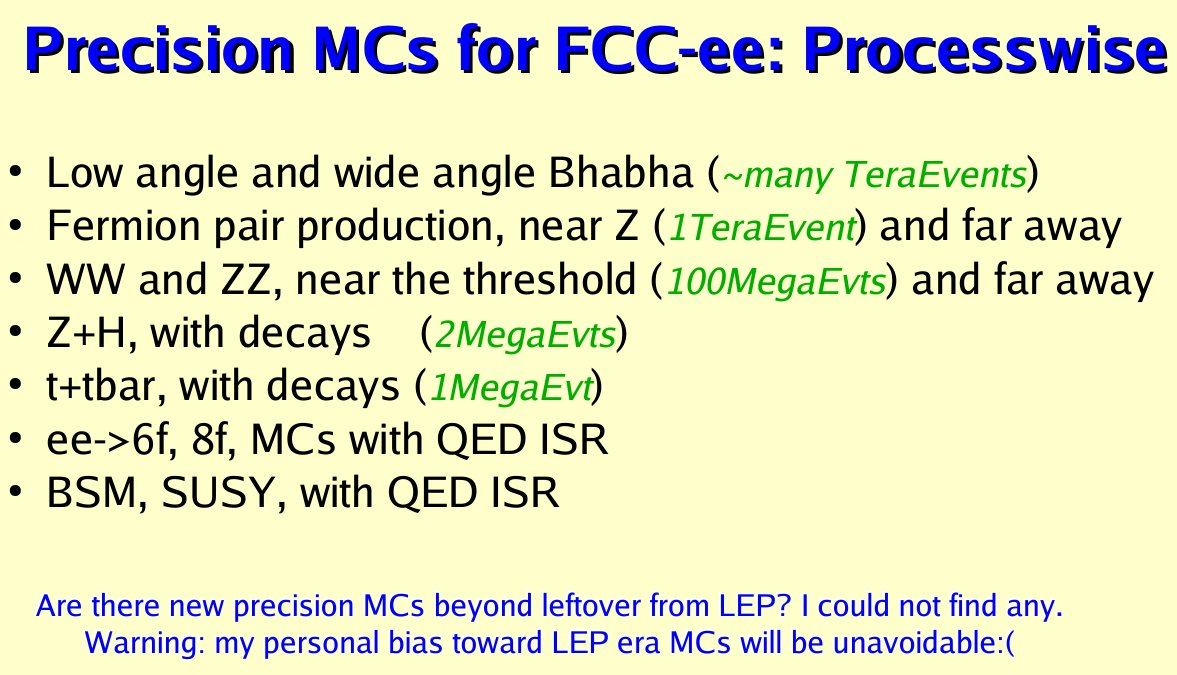
\includegraphics[width=115mm]{./sli2.jpg}
\end{frame}


%----------------------------------------------------------------
%----------------------------------------------------------------
\begin{frame}[fragile]
\frametitle{\bf\ns 
 Main points from CERN June 2014 talk on precision MCs for FCCee}

\vspace{-2mm}
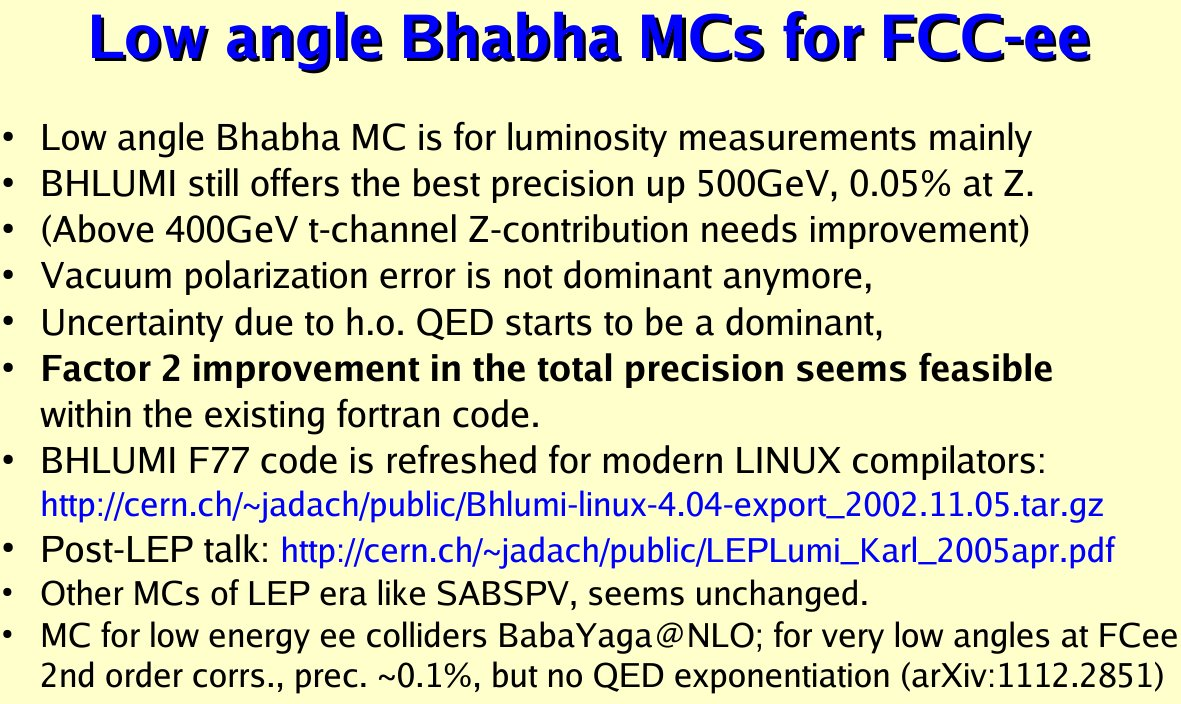
\includegraphics[width=110mm]{./sli4.jpg}

\includegraphics[width=110mm]{./sli5.jpg}
\end{frame}

%----------------------------------------------------------------
%----------------------------------------------------------------
\begin{frame}[fragile]
\frametitle{\bf\ns 
 Main points from CERN June 2014 talk on precision MCs for FCCee}

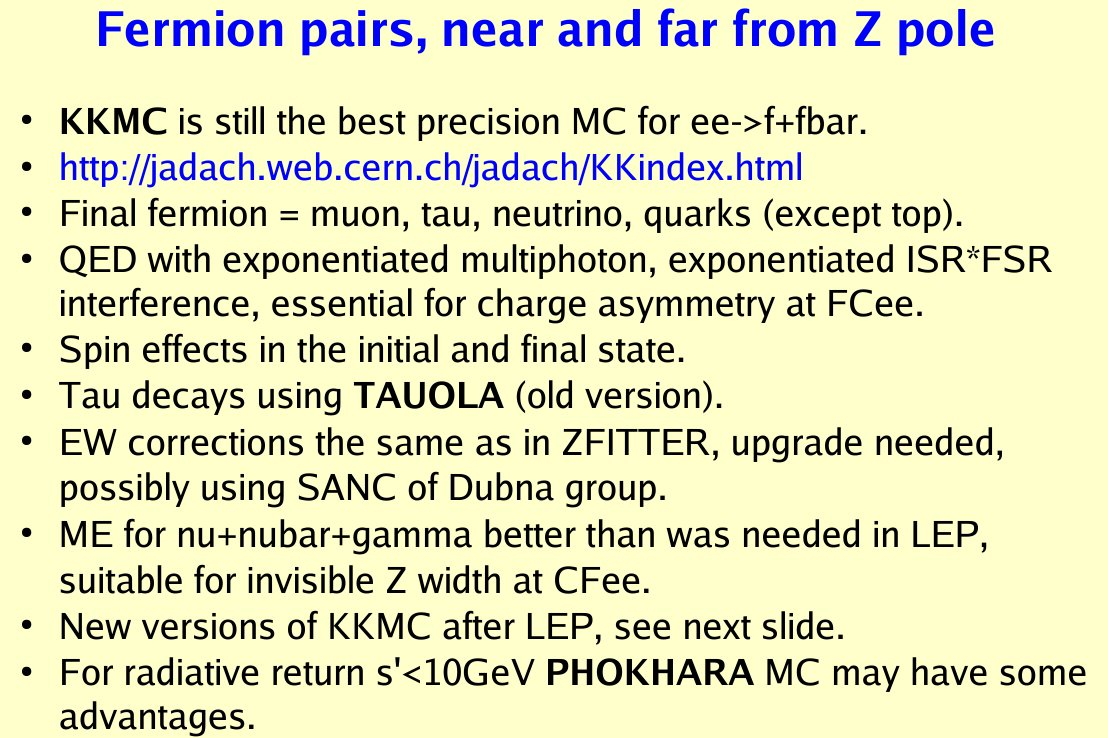
\includegraphics[width=115mm]{./sli6.jpg}
\end{frame}

%----------------------------------------------------------------
%----------------------------------------------------------------
\begin{frame}[fragile]
\frametitle{\bf\ns 
 Main points from CERN June 2014 talk on precision MCs for FCCee}
\framesubtitle{\large\bf\crd WW and ZZ far and near from the threshold}

%\vspace{-2mm}
\begin{itemize}
\item
KORALZ+YFSWW (2002) and YFSZZ for ee -> 4f,
kept alive but little new after LEP (spin correlations added),\\
{\cbl http://placzek.web.cern.ch/placzek/}
\item
KORALW in quadri-precision for ee->eeee revived under LINUX recently.
\item
RacoonWW (2004) stays essentially at the level of LEP,\\
{\cbl http://ltpth.web.psi.ch/racoonww/racoonww.html}
\item
WHIZARD (2014) rather primitive ISR, lacks EW corrections,\\
{\cbl https://whizard.hepforge.org}
\item
GRACE (2006) EW corrections seems to be there, but simplistic QED\\ 
{\cbl http://minami-home.kek.jp}
\item
YFSZZ: main MC for ee->ZZ at LEP\\
{\cbl http://placzek.web.cern.ch/placzek/}
\end{itemize}
\end{frame}


%----------------------------------------------------------------
%----------------------------------------------------------------
\begin{frame}[fragile]
\frametitle{\bf\ns 
 Main points from CERN June 2014 talk on precision MCs for FCCee}
\framesubtitle{\large\bf\crd WW and ZZ far and near from the threshold}

Post-LEP developments:
\begin{itemize}
\item
Important work by Denner, Dittmaier Roth, Wieders:\\
\item
%{\footnotesize
Full ee->WW->4f NLO calculation, with fully off-shell W bosons
(the first 2->4 NLO calculation.) 
It nicely confirms the validity of our older results based on the double-pole approximation at the expected level of accuracy.
%}
\item
Results published http://arxiv.org/abs/hep-ph/0502063, hep-ph/0505042
\item
Limited to WW-like final states like
$u \bar{d}  \mu \bar{\nu}_\mu$.
\item
MC programs not published, QED expon. still missing.
\end{itemize}
Other unfinished work:
\begin{itemize}
\item
Resummation QED interferences for YFSWW MC outlined\\ http://cern.ch/~jadach/public/granada\_2001march.pdf\\
but never implemented (was not needed for LEP2)
\end{itemize}


\end{frame}
%----------------------------------------------------------------

%----------------------------------------------------------------
%----------------------------------------------------------------
\begin{frame}[fragile]
\frametitle{\bf\ns 
 Main points from CERN June 2014 talk on precision MCs for FCCee}

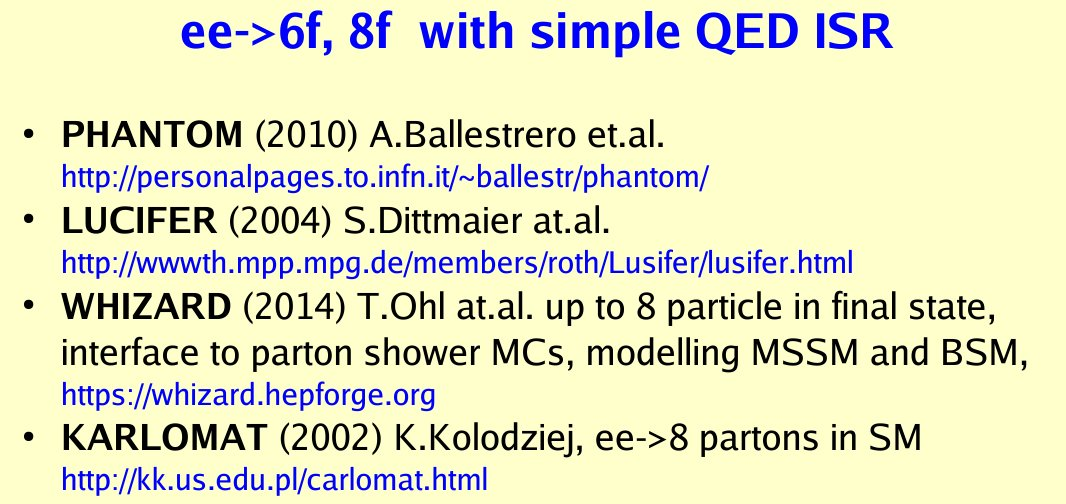
\includegraphics[width=115mm]{./sli10.jpg}
\end{frame}
%----------------------------------------------------------------


%----------------------------------------------------------------
%----------------------------------------------------------------
\begin{frame}[fragile]
\frametitle{\bf\ns 
 Main points from CERN June 2014 talk on precision MCs for FCCee}

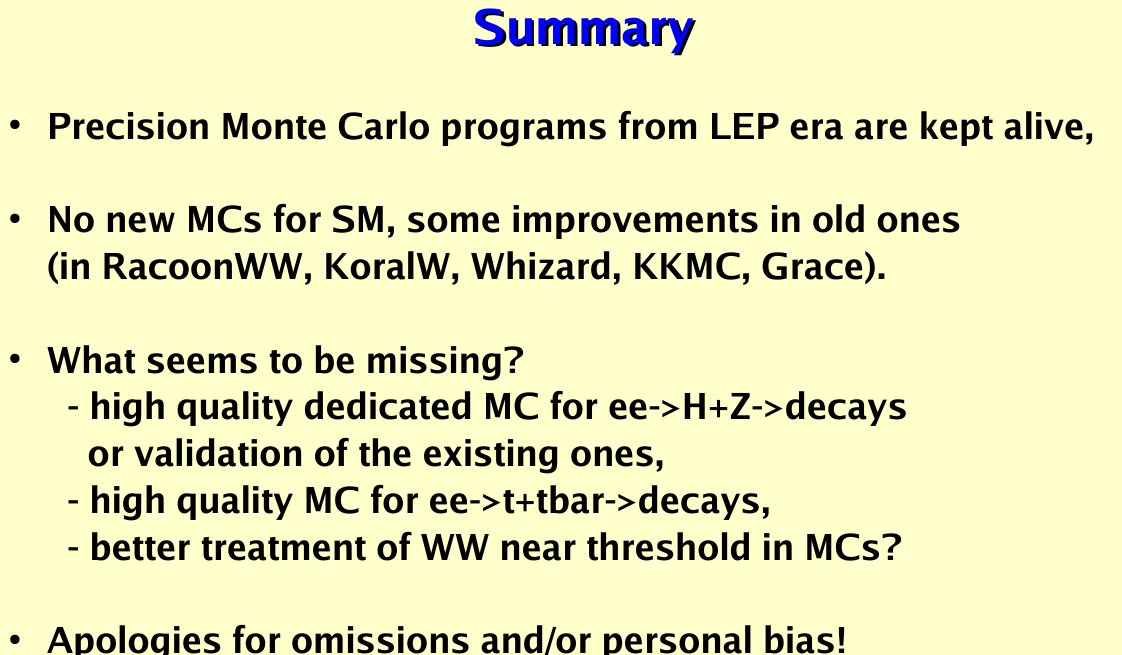
\includegraphics[width=115mm]{./sli12.jpg}
\end{frame}
%----------------------------------------------------------------



%----------------------------------------------------------------
%----------------------------------------------------------------
%----------------------------------------------------------------
%----------------------------------------------------------------
%----------------------------------------------------------------
%----------------------------------------------------------------
\begin{frame}[fragile]
\frametitle{\bf New wiki page of MC generators for FCCee}
\framesubtitle{\bf http://192.245.169.66:8000/FCCeeMC/wiki}

\begin{itemize}
\item
 Actual location on the cloud cluster at IFJ PAN is most likely
 temporary -- we may move it to {\bf hepforge}
\item
 For the moment it includes undusted KKMC and BHLUMI,
 with reanimated makefiles (compile/run) under SLC5
\item
 More to be put there:
\begin{itemize}
\item Other post-LEP programs (KORALW, YFSWW, YFSZZ, BHWIDE)
\item Link to other repositories, RacoonWW?
\item Some new codes, for instance ISR to Higgs lineshape...
\item Selected/relevant presentations
\end{itemize}
\item\crd
 {\bf The rule} will be that we include only codes which run
 under modern compilators 
 and are supplied with simple instruction 
 how to start working with them!
\end{itemize}
\end{frame}

%----------------------------------------------------------------
%----------------------------------------------------------------
\begin{frame}[fragile]
\frametitle{\bf New wiki page of MC generators for FCCee}
\framesubtitle{\bf http://192.245.169.66:8000/FCCeeMC/wiki}

Many thanks to Andrzej Siodmok and Mariusz Witek\\
for help in setting up wiki system on\\
the Cracow Cloud One cluster at IFJ PAN, Krakow!

\vspace{3mm}

\includegraphics[width=105mm]{./wiki_cc1.jpg}

\end{frame}

%----------------------------------------------------------------
\begin{frame}[fragile]
\frametitle{\bf New wiki page of MC generators for FCCee}
\framesubtitle{\bf http://192.245.169.66:8000/FCCeeMC/wiki}

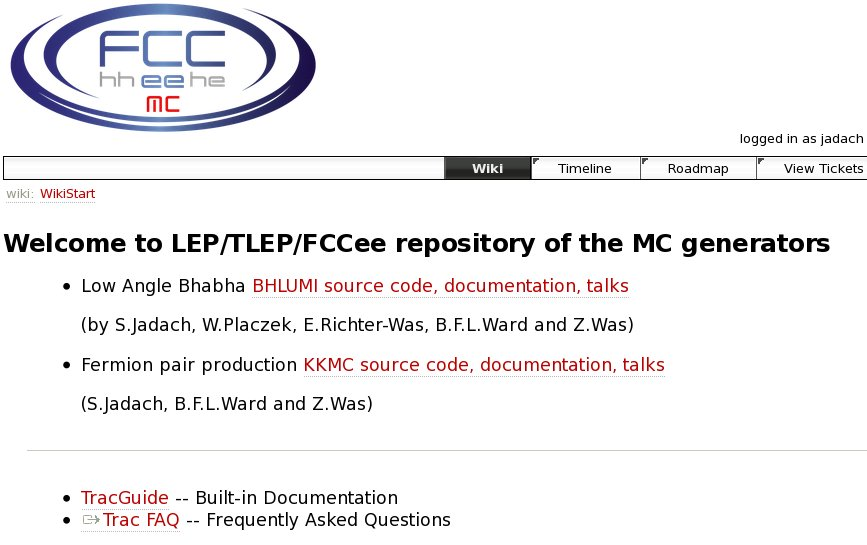
\includegraphics[width=118mm]{./wiki0.jpg}
%%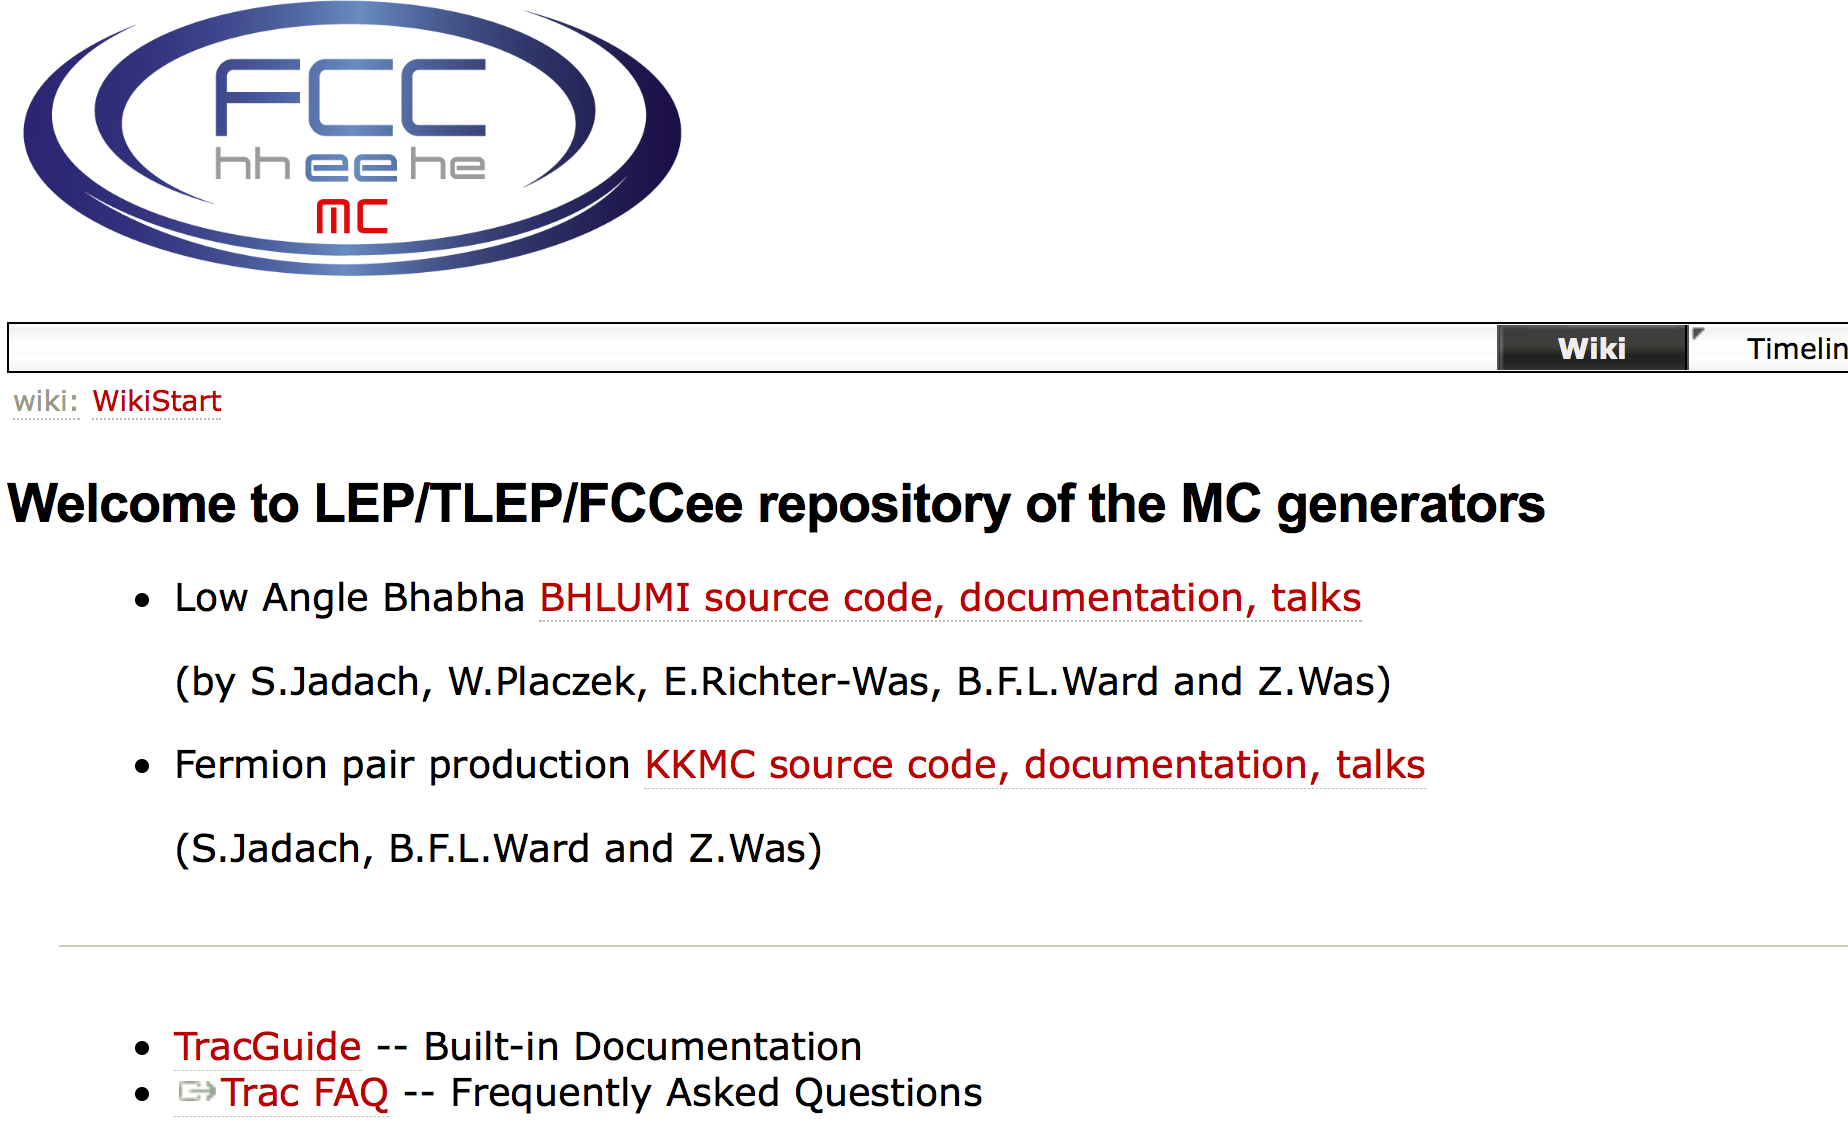
\includegraphics[width=120mm]{./wiki0.png}

\end{frame}

%----------------------------------------------------------------
%----------------------------------------------------------------
\begin{frame}[fragile]
\frametitle{\bf New wiki page of MC generators for FCCee}
\framesubtitle{\bf BHLUMI at http://192.245.169.66:8000/FCCeeMC/wiki}

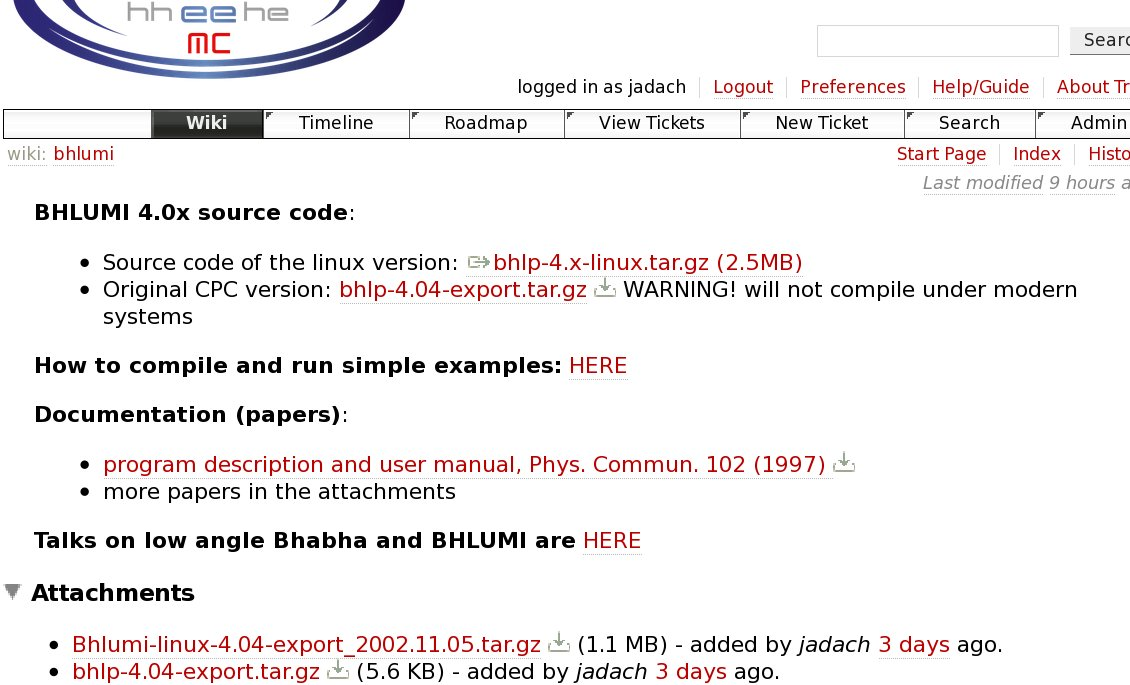
\includegraphics[width=118mm]{./wiki1.jpg}

\end{frame}
%----------------------------------------------------------------


%----------------------------------------------------------------
%----------------------------------------------------------------
\begin{frame}[fragile]
\frametitle{\bf New wiki page of MC generators for FCCee}
\framesubtitle{\bf BHLUMI subpage 1 }

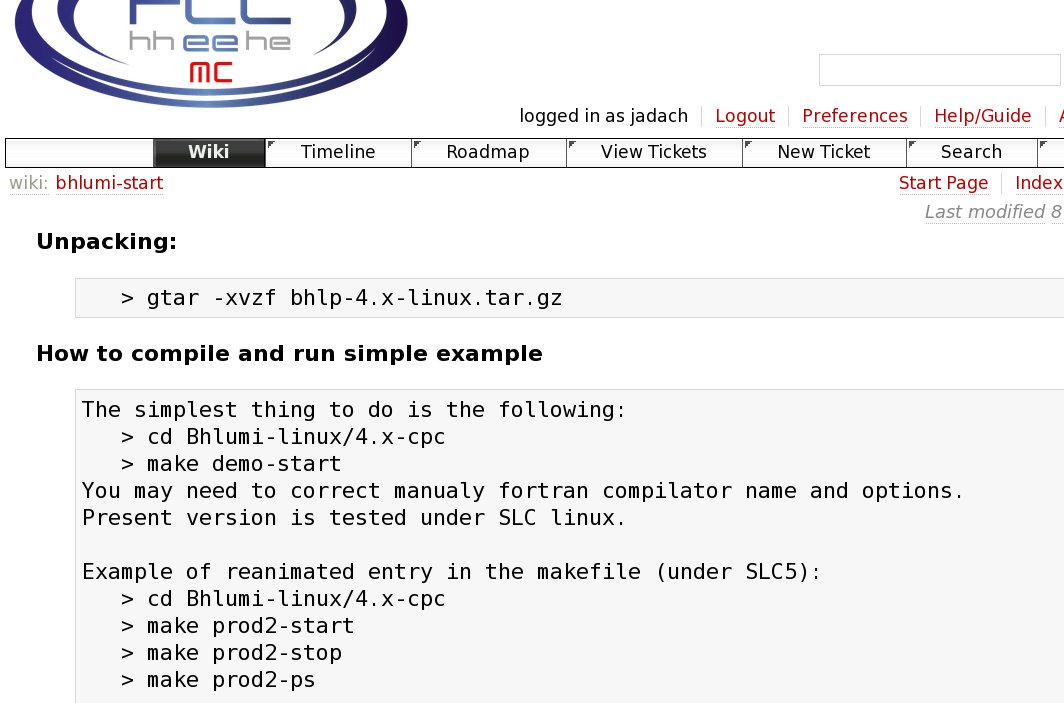
\includegraphics[width=118mm]{./wiki2.jpg}

\end{frame}


%----------------------------------------------------------------
%----------------------------------------------------------------
\begin{frame}[fragile]
\frametitle{\bf New wiki page of MC generators for FCCee}
\framesubtitle{\bf BHLUMI subpage 2}

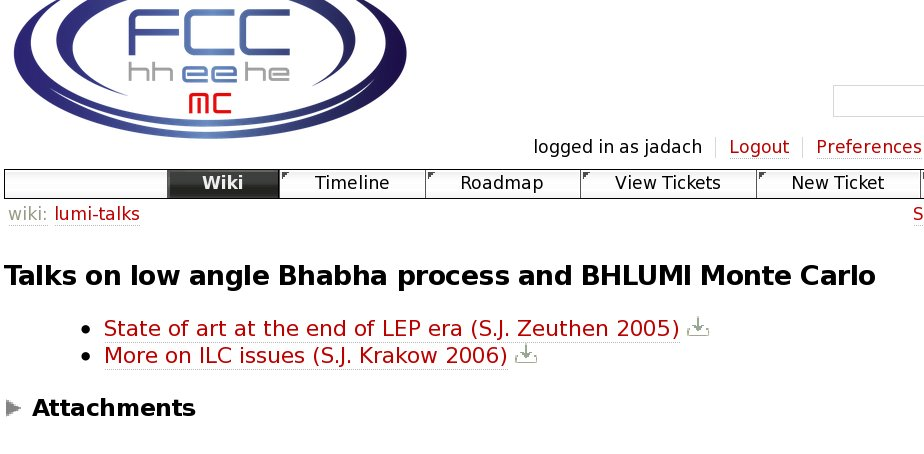
\includegraphics[width=118mm]{./wiki3.jpg}

\end{frame}

%----------------------------------------------------------------
%----------------------------------------------------------------
\begin{frame}[fragile]
\frametitle{\bf New wiki page of MC generators for FCCee}
\framesubtitle{\bf KKMC main page on wiki}

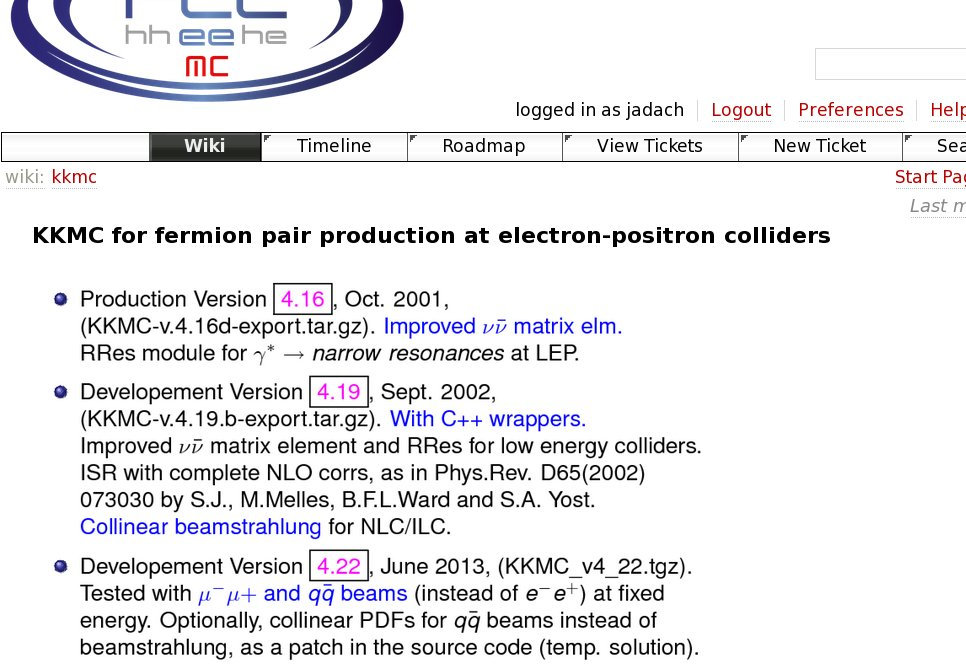
\includegraphics[width=110mm]{./wiki0k.jpg}

\end{frame}

%----------------------------------------------------------------
%----------------------------------------------------------------
\begin{frame}[fragile]
\frametitle{\bf New wiki page of MC generators for FCCee}
\framesubtitle{\bf KKMC main page on wiki}

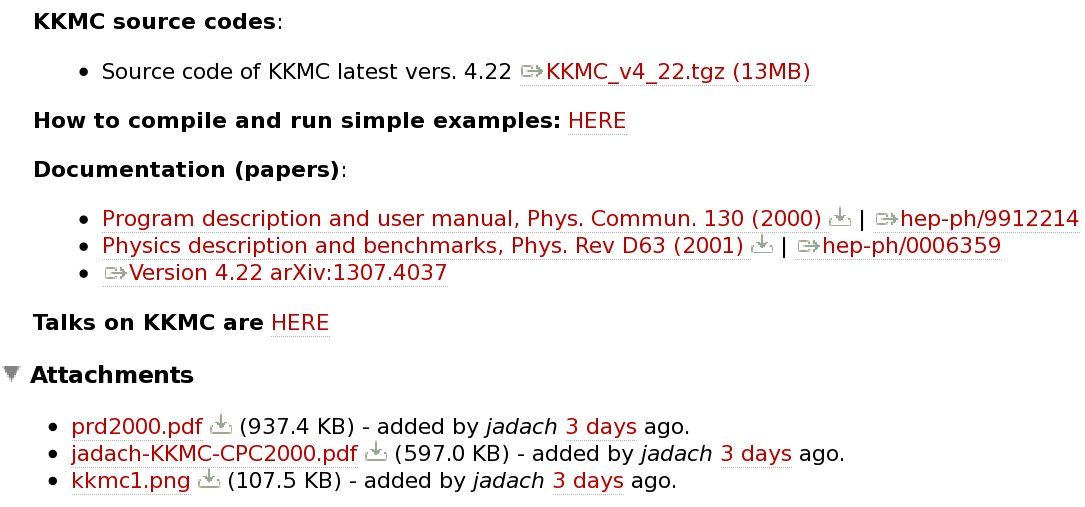
\includegraphics[width=120mm]{./wiki1k.jpg}

\end{frame}



%----------------------------------------------------------------
%----------------------------------------------------------------
\begin{frame}[fragile]
\frametitle{\bf New wiki page of MC generators for FCCee}
\framesubtitle{\bf KKMC user instruction 1}

\vspace{-3mm}
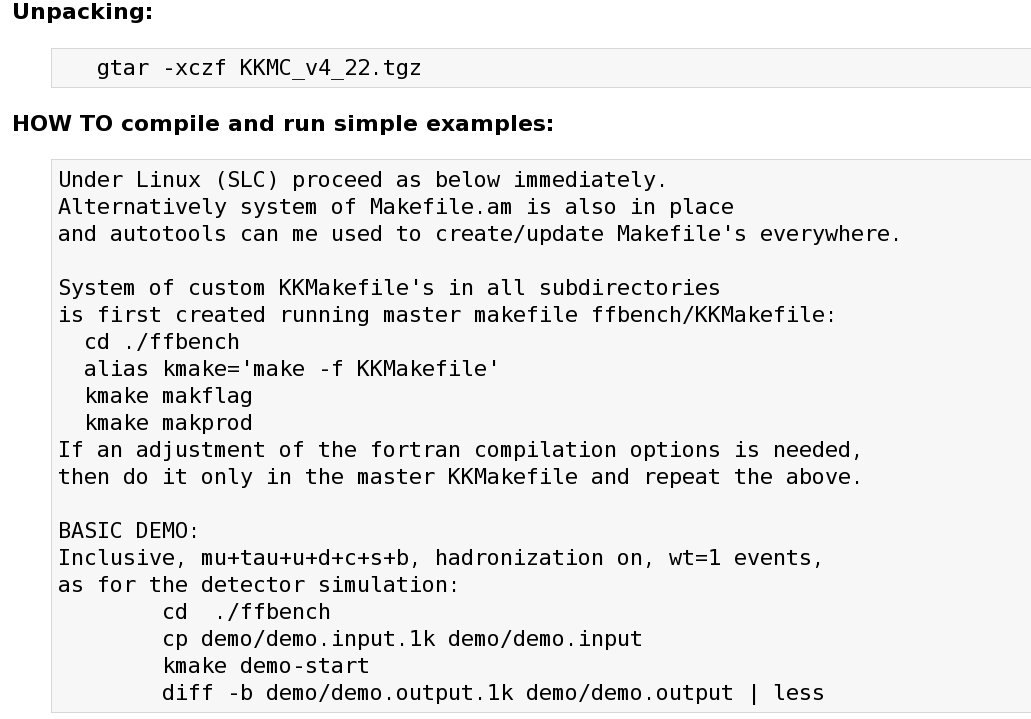
\includegraphics[width=115mm]{./wiki2k.jpg}

\end{frame}


%----------------------------------------------------------------
%----------------------------------------------------------------
\begin{frame}[fragile]
\frametitle{\bf New wiki page of MC generators for FCCee}
\framesubtitle{\bf KKMC user instruction 2}

\vspace{-3mm}
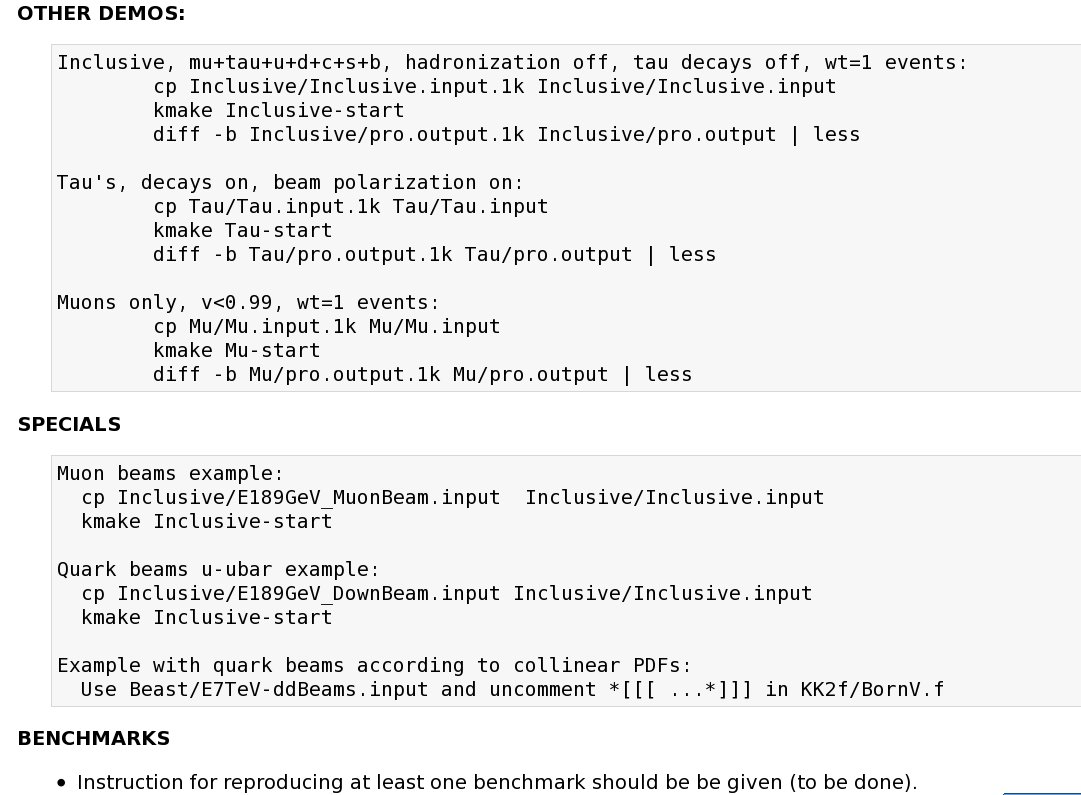
\includegraphics[width=110mm]{./wiki3k.jpg}

\end{frame}

\begin{frame}[fragile]
\frametitle{\bf New wiki page of MC generators for FCCee}
\framesubtitle{\bf http://192.245.169.66:8000/FCCeeMC/wiki}

\begin{itemize}
\item
 More post-LEP MC's will be put there.
\item 
 Only codes which run under modern (linux) systems
 and are supplied with simple instructions
 will be admitted!
\item
 In principle codes from non-Krakow will be allowed...
\item
 Actual location may be temporary -- moving to hepforge?
\end{itemize}
\end{frame}

%----------------------------------------------------------------
%----------------------------------------------------------------
%----------------------------------------------------------------
%----------------------------------------------------------------
%----------------------------------------------------------------
%----------------------------------------------------------------
\begin{frame}[fragile]
\frametitle{\bf Update on invisible Z width from radiative return}
\framesubtitle{\bf\crd\large Event selection criteria in the MC exercise}

Accepted $\nu\bar\nu+n\gamma$ and $\mu^-\mu^+ +n\gamma$ events:
\begin{itemize}
\item 
One or more photons seen with:\\
$\theta_\gamma >15^{\circ}$,
$E_\gamma/E_{beam}>0.10$ and $p^T_\gamma/E_{beam}>0.02$
\item
Muon pair within the angular range $\cos\theta_{\pm}<0.95$
\end{itemize}
MC events were generated using KKMC.

\end{frame}


%----------------------------------------------------------------
%----------------------------------------------------------------
\begin{frame}[fragile]
\frametitle{\bf Update on invisible Z width from radiative return}
\framesubtitle{\bf\large Selection criteria at work 161GeV}

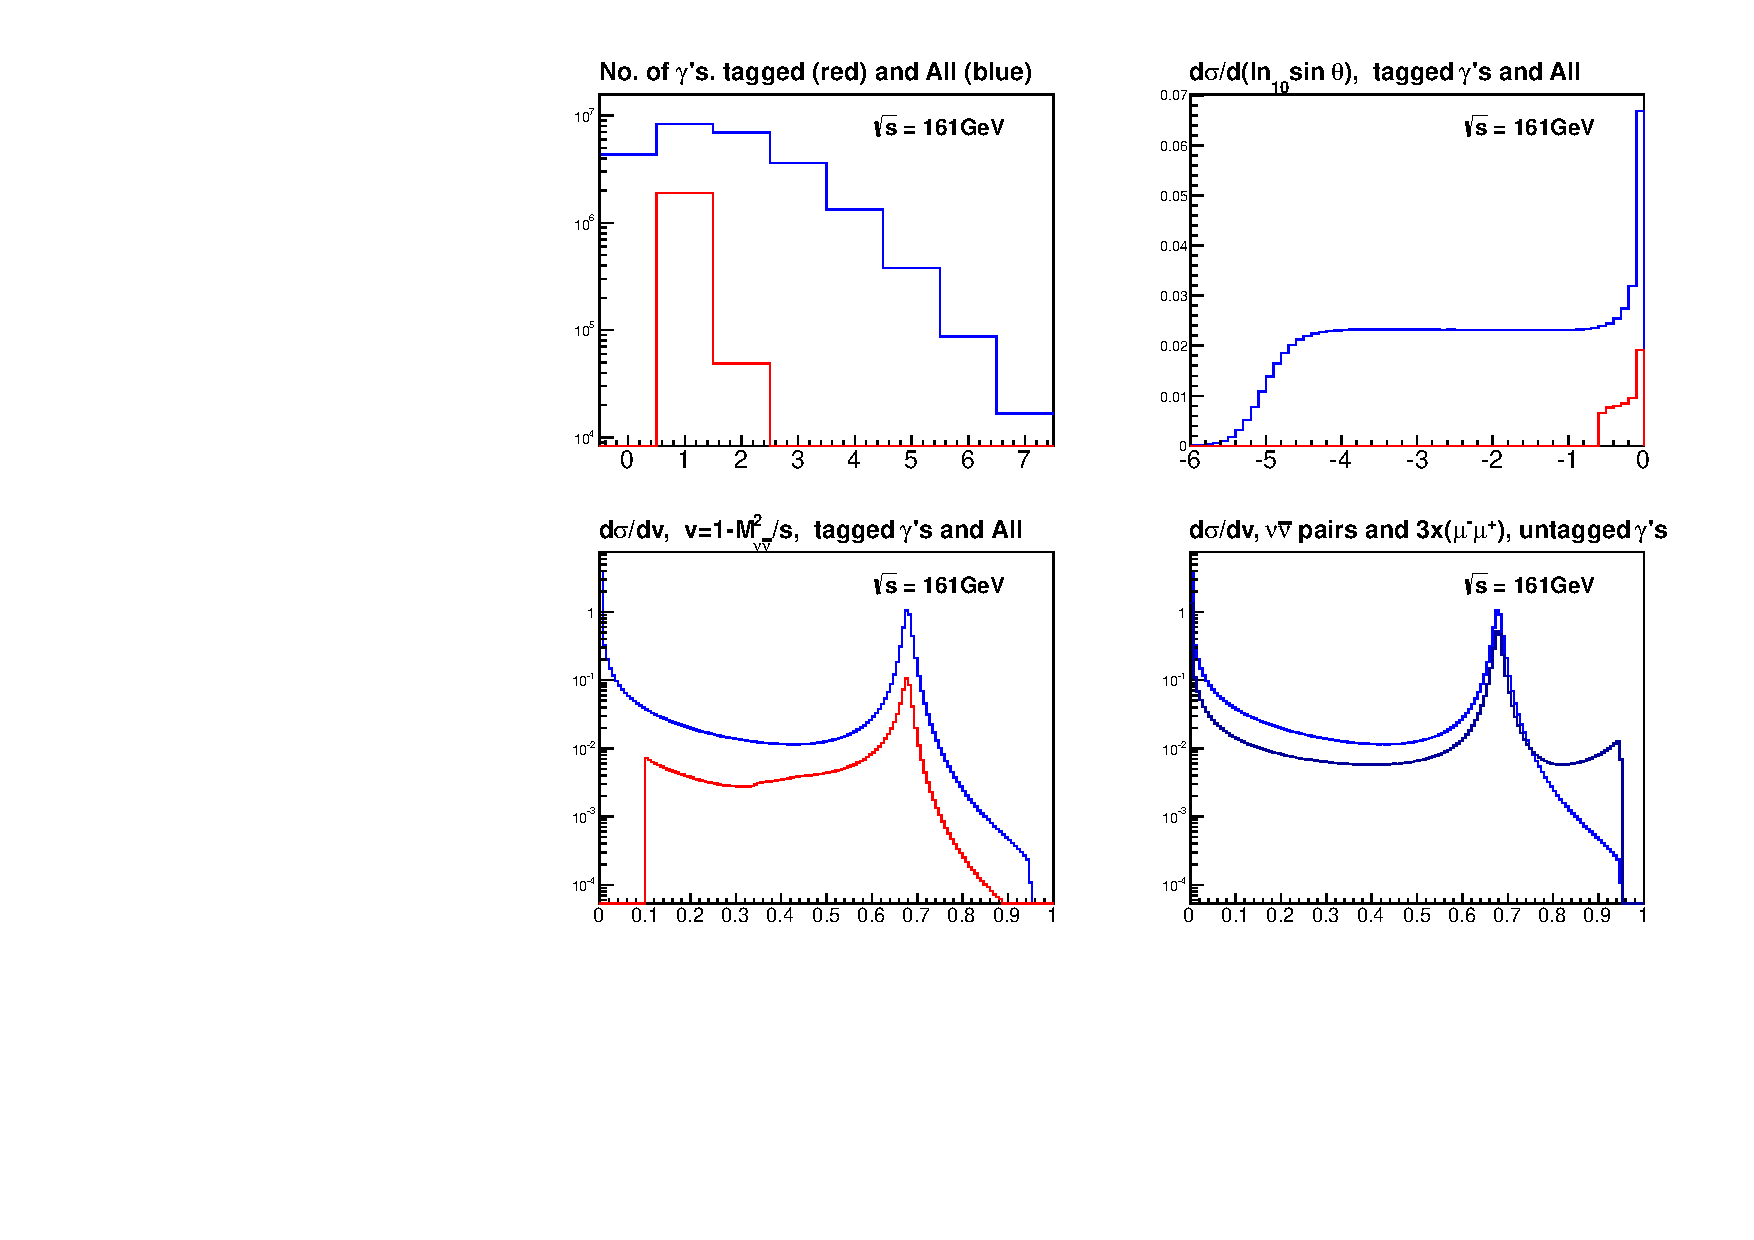
\includegraphics[width=110mm,height=80mm]{./cFigInfo_E161.pdf}
\end{frame}
%----------------------------------------------------------------

%----------------------------------------------------------------
\begin{frame}[fragile]
\frametitle{\bf Update on invisible Z width from radiative return}
\framesubtitle{\bf\large Selection criteria at work 105GeV}

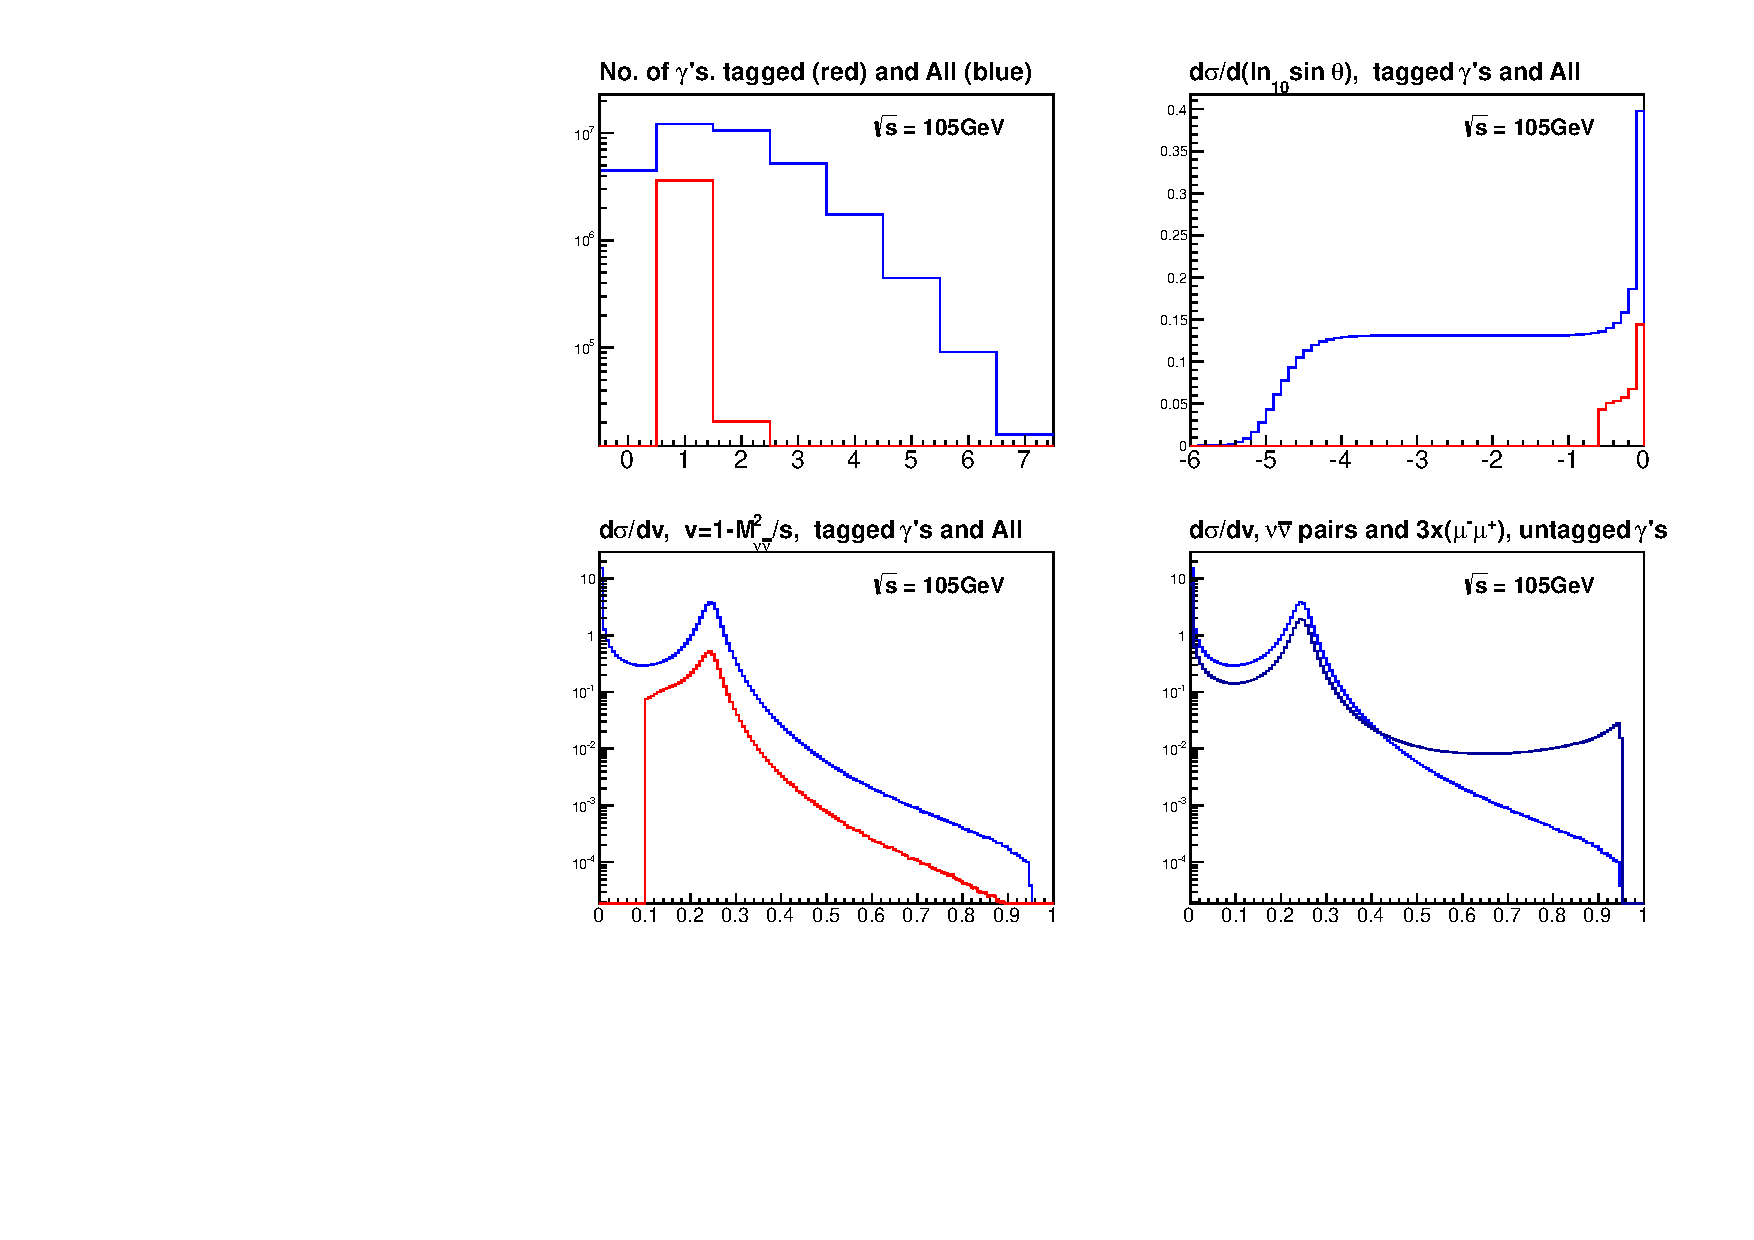
\includegraphics[width=110mm,height=80mm]{./cFigInfo_E105.pdf}
\end{frame}


%----------------------------------------------------------------
%----------------------------------------------------------------
\begin{frame}[fragile]
\frametitle{\bf Update on invisible Z width from radiative return}
\framesubtitle{\bf\large t-channel contribution at 161GeV}

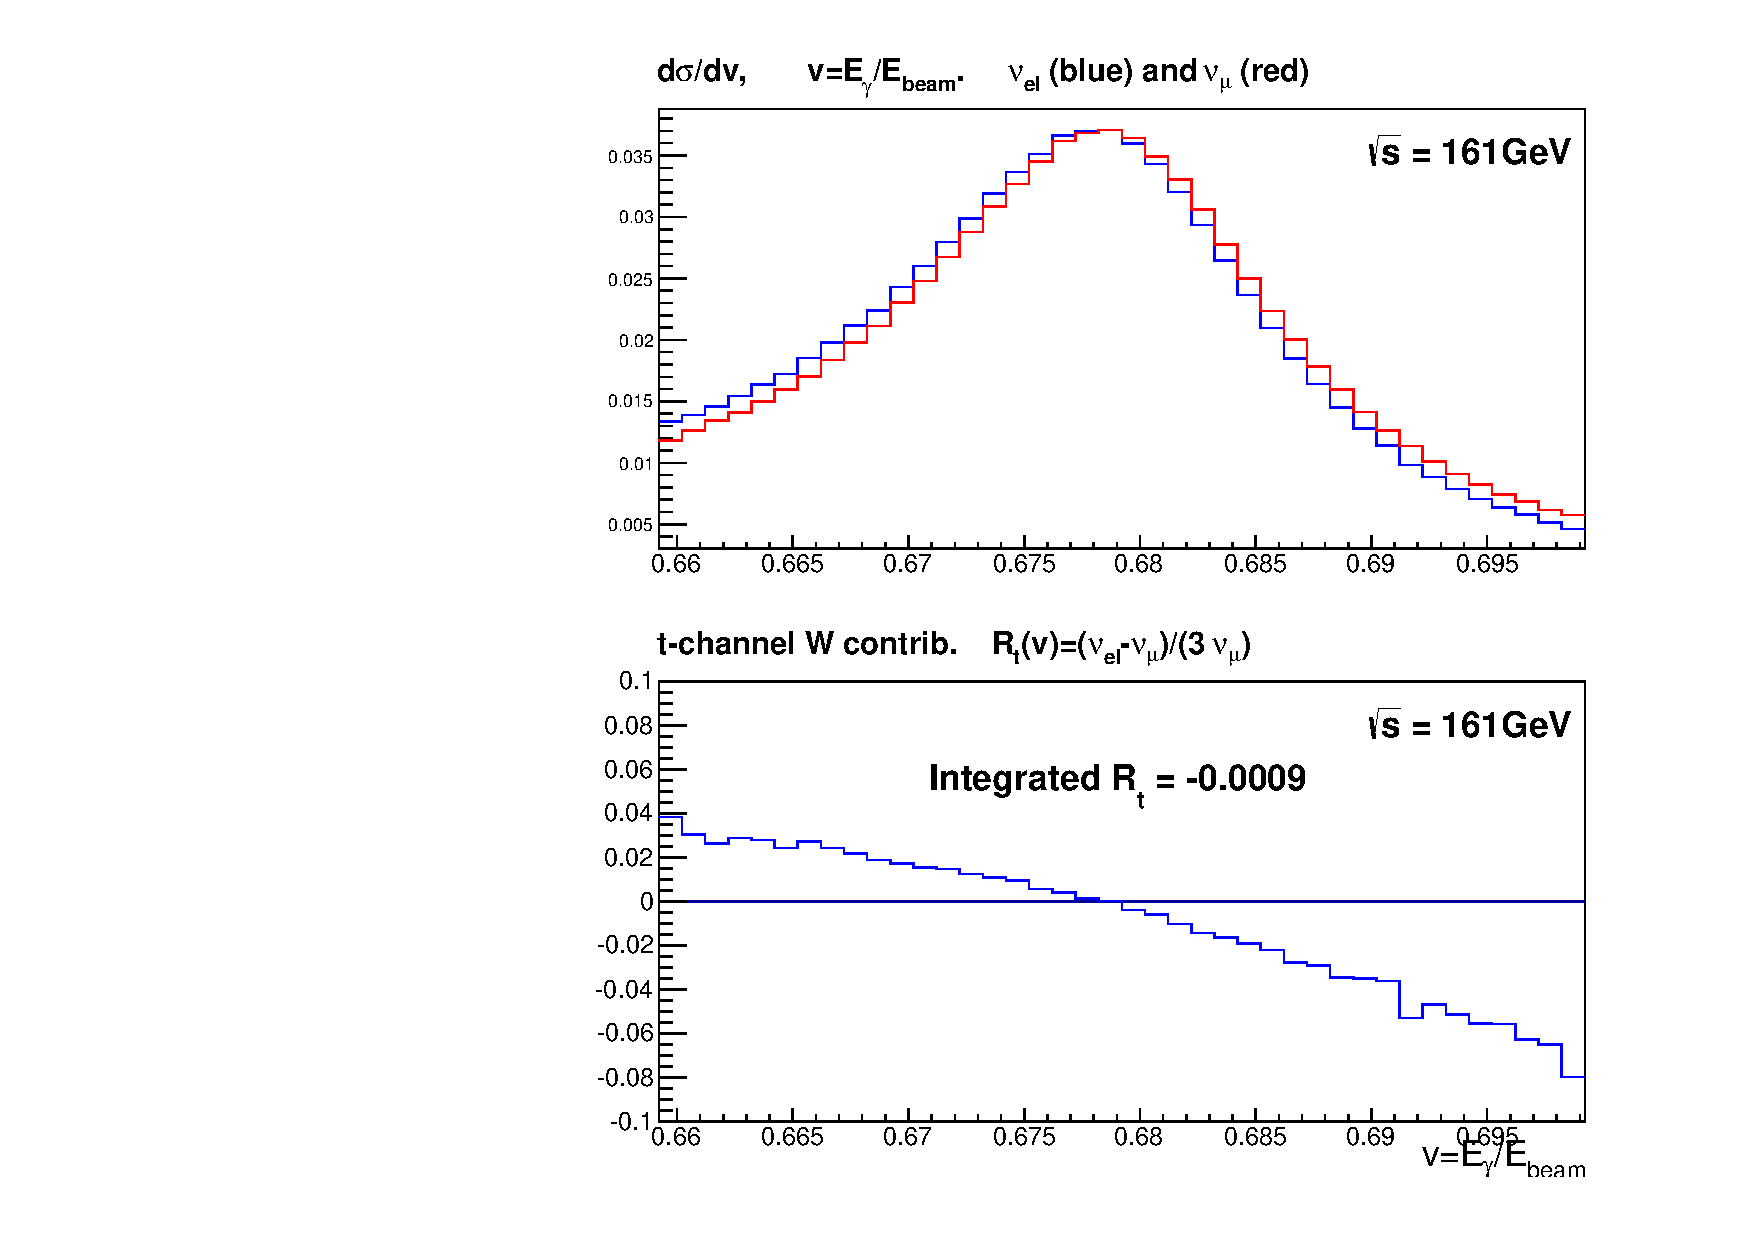
\includegraphics[width=110mm,height=80mm]{./cNuDiff_E161.pdf}
\end{frame}

%----------------------------------------------------------------
%----------------------------------------------------------------
\begin{frame}[fragile]
\frametitle{\bf Update on invisible Z width from radiative return}
\framesubtitle{\bf\large t-Chanel contribution at 161GeV}

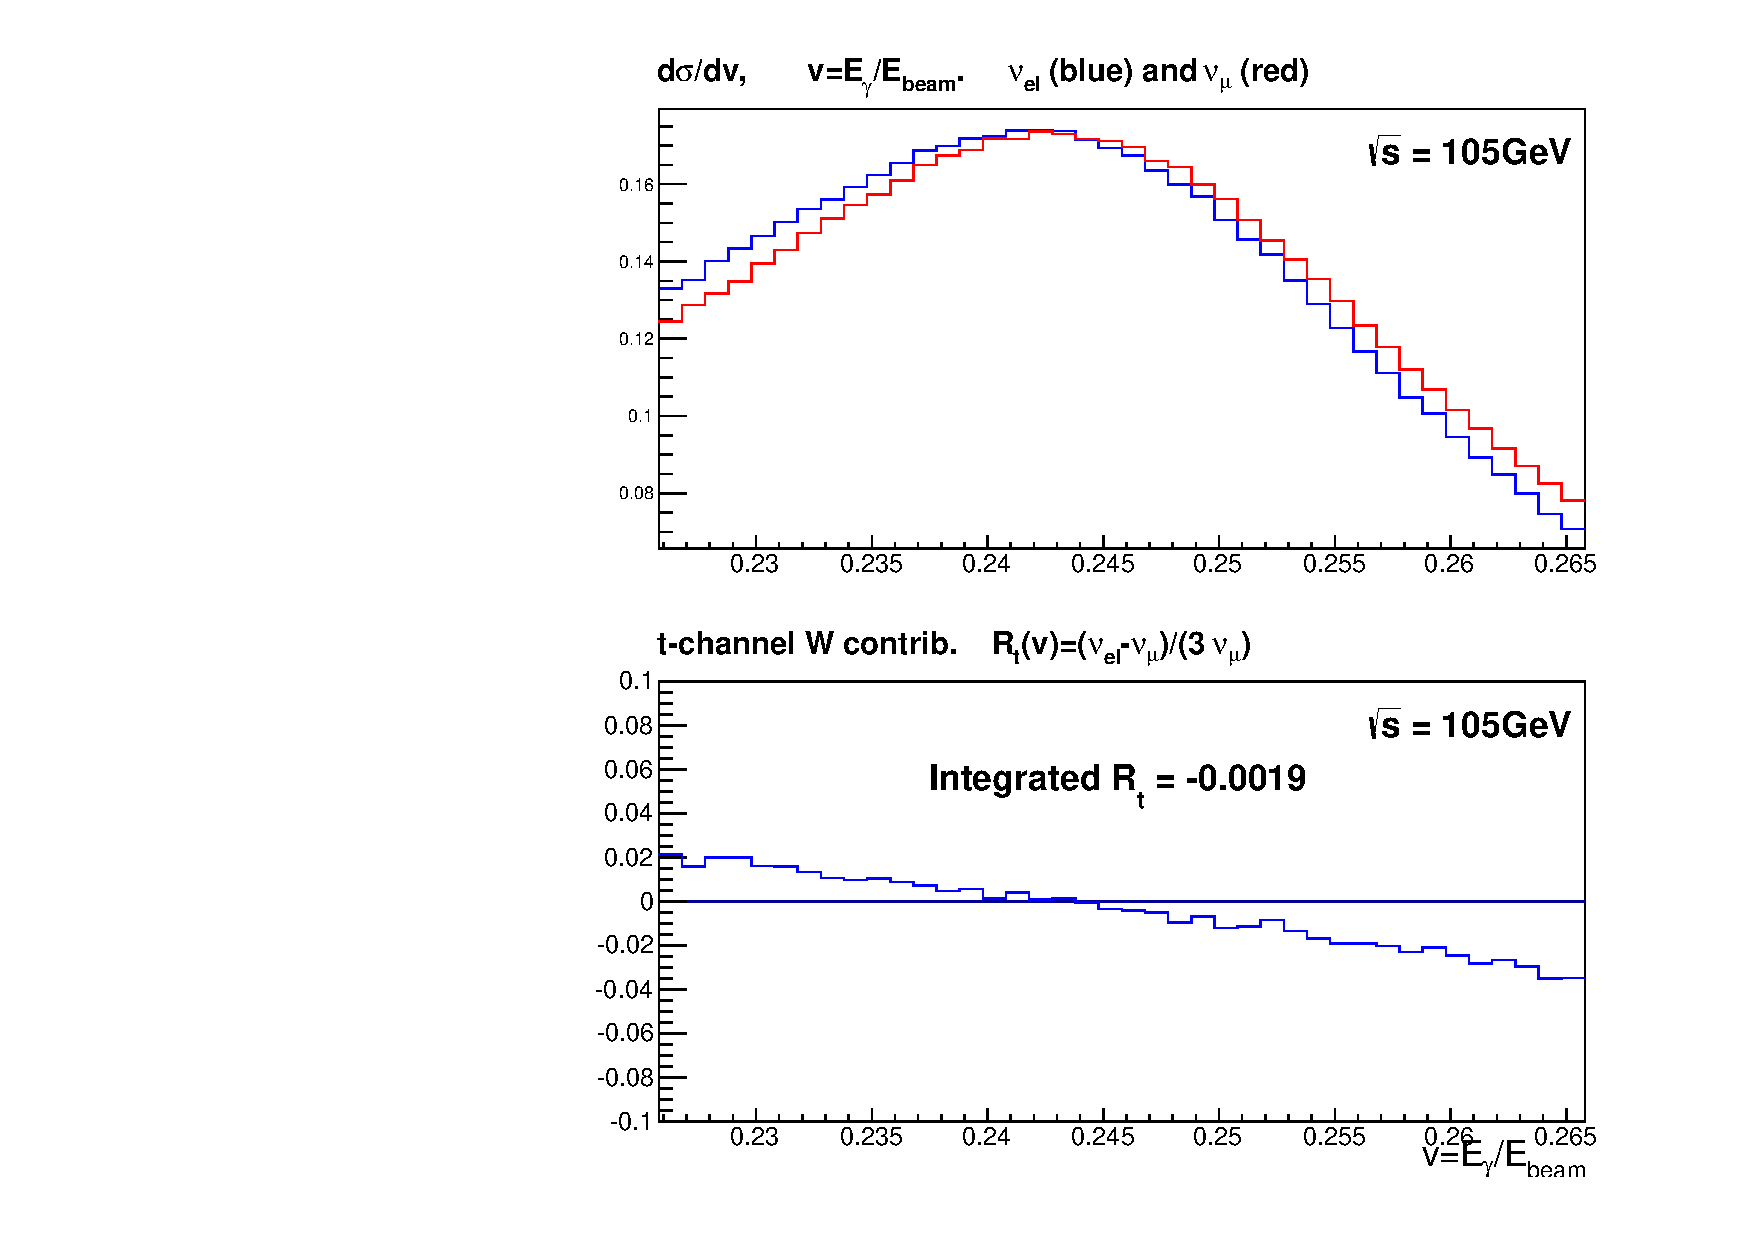
\includegraphics[width=110mm,height=80mm]{./cNuDiff_E105.pdf}
\end{frame}


%----------------------------------------------------------------
%----------------------------------------------------------------
\begin{frame}[fragile]
\frametitle{\bf Update on invisible Z width from radiative return}
\framesubtitle{\bf\large h.o. QED at 161GeV}

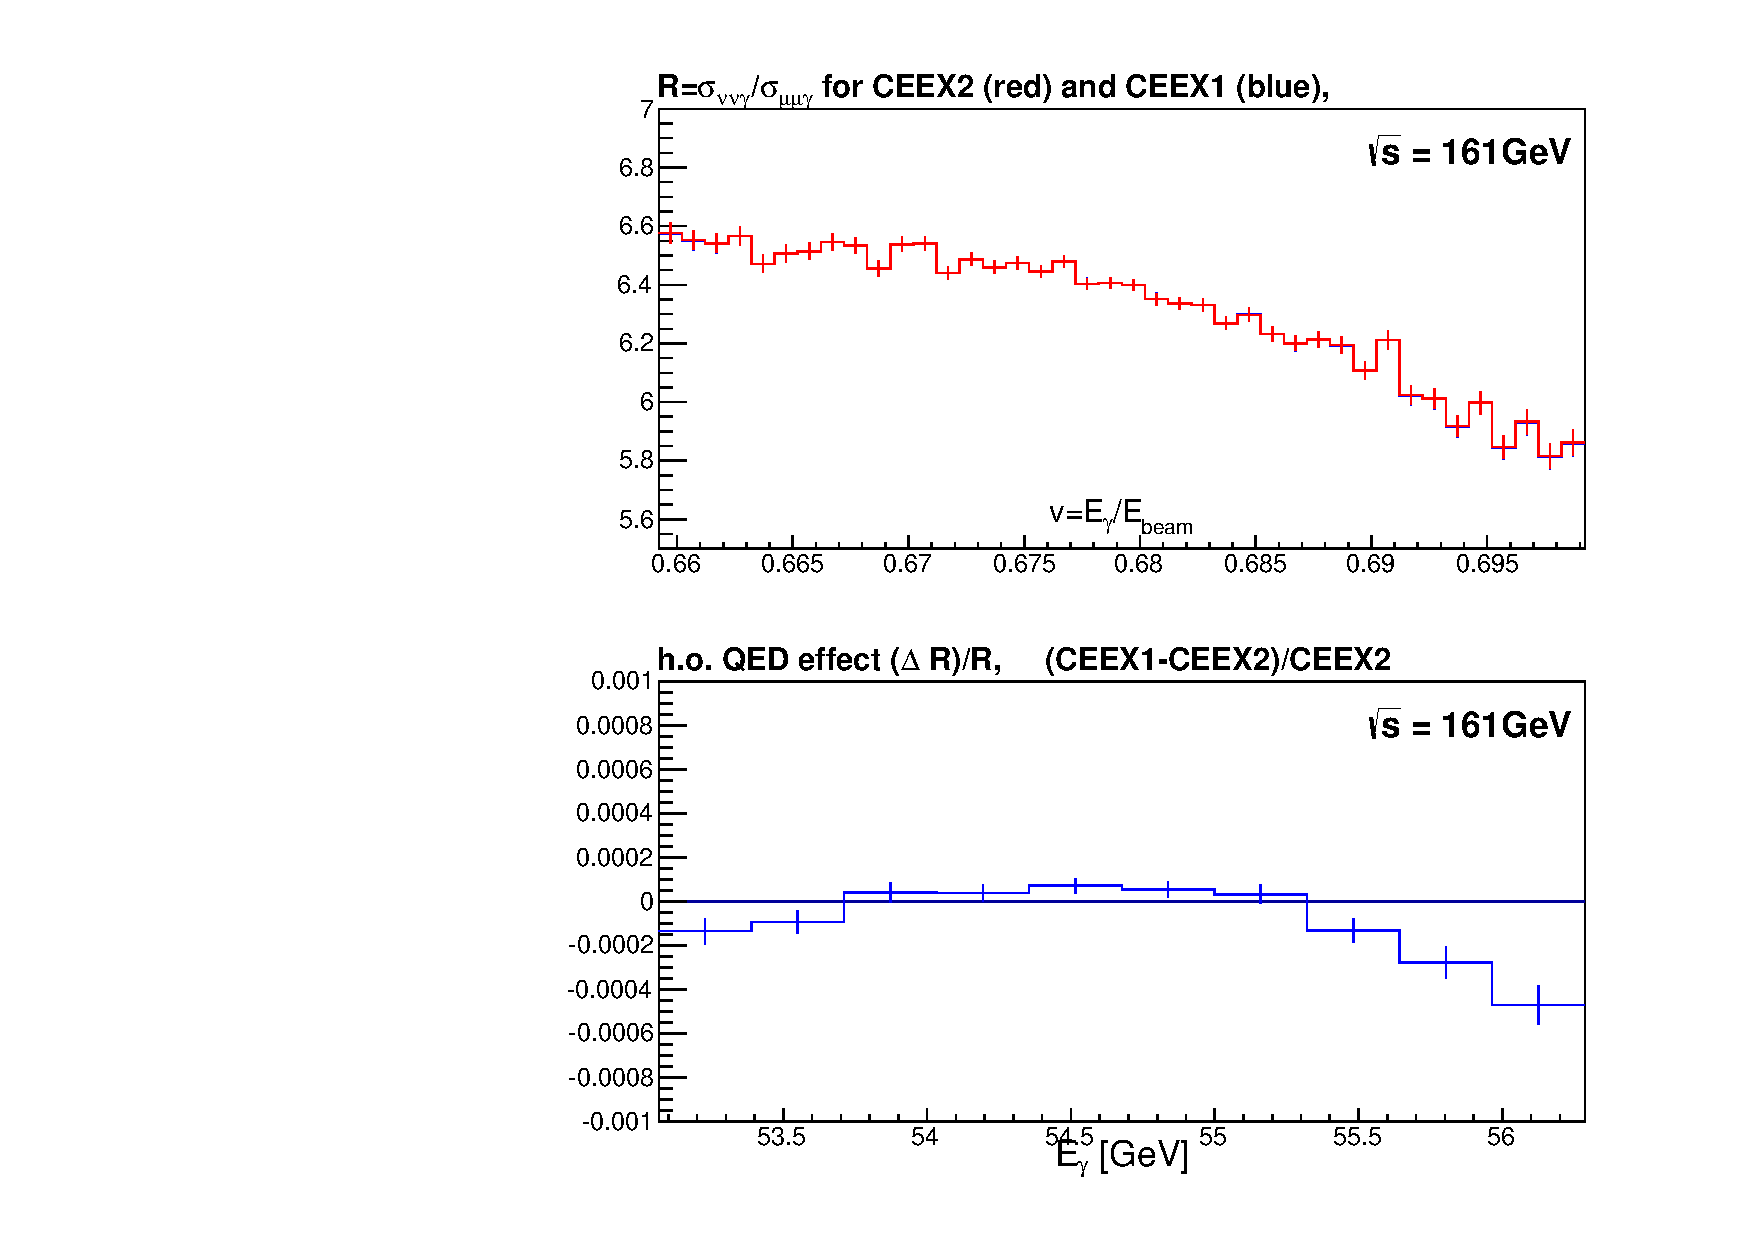
\includegraphics[width=110mm,height=80mm]{./cCeex21rat_E161.pdf}
\end{frame}

%----------------------------------------------------------------
%----------------------------------------------------------------
\begin{frame}[fragile]
\frametitle{\bf Update on invisible Z width from radiative return}
\framesubtitle{\bf\large h.o. QED at 105GeV}

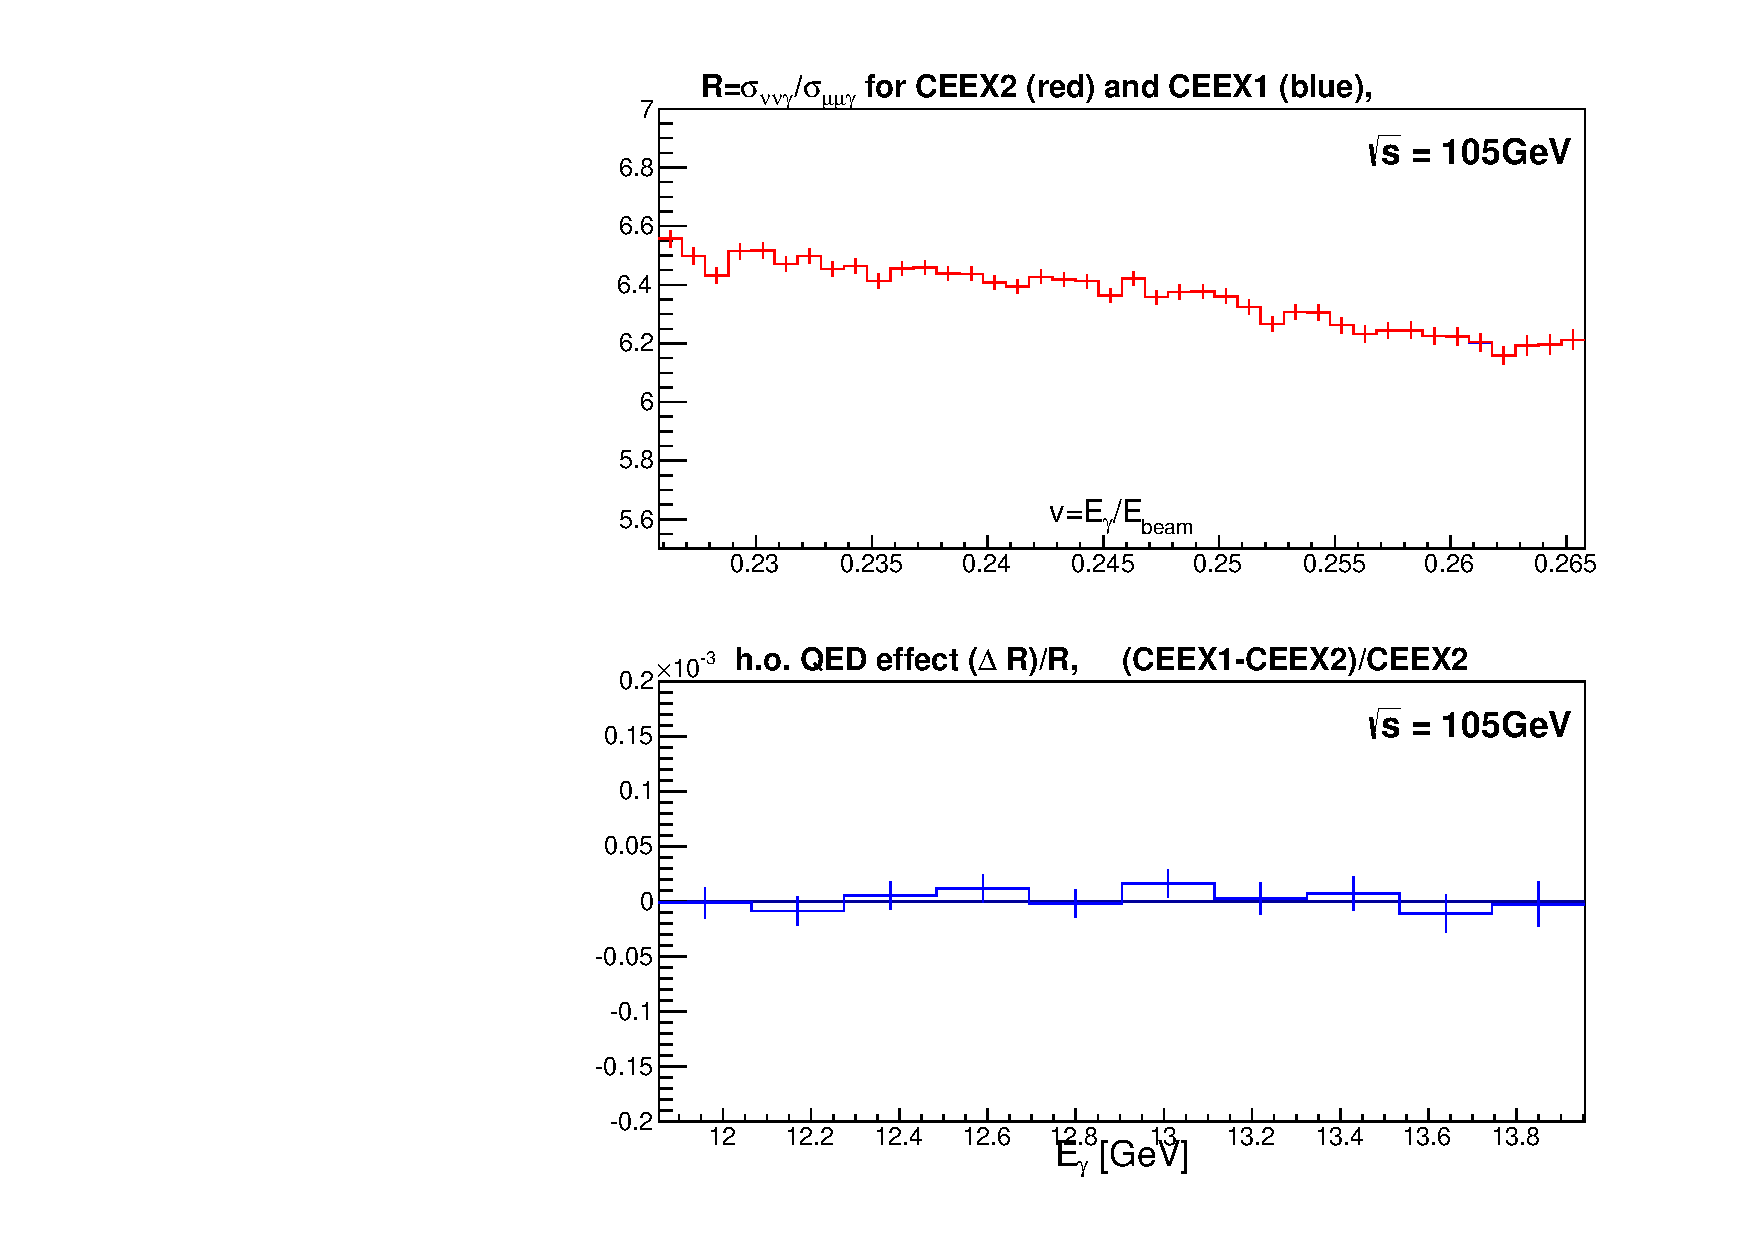
\includegraphics[width=110mm,height=80mm]{./cCeex21rat_E105.pdf}
\end{frame}


%----------------------------------------------------------------
%----------------------------------------------------------------
\begin{frame}[fragile]
\frametitle{\bf Update on invisible Z width from radiative return}

{\bf Today's conclusions on invisible Z:}
\begin{itemize}
\item 
 QED h.o. corrections very small $\sim 10^{-4}$
\item
 t-Chanel W exchange contrib intergrated over Z-peak
 much smaller than expected: $\sim 10^{-3}$
\item
 Both twice smaller at 105GeV than at 161GeV
\item
 More studies are needed.
\item
 In particular which QED H.O. diagrams are most important.
\end{itemize}
\end{frame}

\end{document}
%%%%%%%%%%%%%%%%%%%%%%%%%%%%%%%%%%%%%%%%%%%%%%%%%%%%%%%%%%%%%%%%%%
%%%%%%%%%%%%%%%%%%%%%%%%%%%%%%%%%%%%%%%%%%%%%%%%%%%%%%%%%%%%%%%%%%
%%%%%%%%%%%%%%%%%%%%%%%%%%%%%%%%%%%%%%%%%%%%%%%%%%%%%%%%%%%%%%%%%%
%%%%%%%%%%%%%%%%%%%%%%%%%%%%%%%%%%%%%%%%%%%%%%%%%%%%%%%%%%%%%%%%%%

-


